\documentclass[10pt]{article}

% Defining page margins
\usepackage[top=1in, bottom=1.5in, left=1in, right=1in]{geometry}
% Ability to generate urls
\usepackage{hyperref}
% Ability to display pseudocode
\usepackage{algorithm}
\usepackage[noend]{algpseudocode}
% Nice graphs
\usepackage{tikz}
% Nice arrows for directed graphs
\usetikzlibrary{arrows.meta,arrows}
% Define colors + coloring cells o tables
\usepackage{color, colortbl}
% Text over right arrow (see: http://tex.stackexchange.com/questions/103988/rightarrow-with-text-above-it)
\usepackage{mathtools}

% Ability to create cells with few lines of text
% see: http://tex.stackexchange.com/questions/2441/how-to-add-a-forced-line-break-inside-a-table-cell
\newcommand{\specialcell}[2][c]{%
  \begin{tabular}[#1]{@{}l@{}}#2\end{tabular}}
  
% Align comment in the same way as Stetements in pseudocode
% see: http://tex.stackexchange.com/questions/74880/algorithmicx-package-comments-on-a-single-line
\algnewcommand{\LineComment}[1]{\State \indent \(\triangleright\) #1}
  
\definecolor{Gray}{gray}{0.9}

% Put arrow in the center of the line
% http://tex.stackexchange.com/questions/39278/tikz-arrowheads-in-the-center
\usetikzlibrary{decorations.markings}
\tikzset{->-/.style={decoration={
  markings,
  mark= at position #1 with {\arrow{Latex[length=4mm]}}},postaction={decorate}}
}

% Nice boxes, which could be used for examples: http://tex.stackexchange.com/questions/74126/beamer-style-text-box
\usepackage{tcolorbox}

% Needed for equation with cases: http://tex.stackexchange.com/questions/47170/how-to-write-conditional-equations-with-one-sided-curly-brackets
\usepackage{amsmath}

\begin{document}

\title{Inference of chemical compound types \\ using graph of chemical reactions}
\author{Yurii Lahodiuk \\ yura.lagodiuk@gmail.com}
\date{}
\maketitle

\begin{abstract}
% TODO: refactor
The fact of participation of chemical compound in some specific chemical reaction - might be treated as implicit signal about properties of given chemical compound. So, in this article, we will consider model for unification of information about multiple chemical reactions in form of graph - for purpose of inference of properties of multiple chemical compounds, using only information about structure of the network (and few additional restrictions). It's become possible, based on results of exploration of properties of chemical reactions graph. And, finally, I would like to provide detailed description of developed programming framework for approximate inference over pairwise Markov Random Fields\cite{project_on_github}.
\end{abstract}

\section{Problem statement}
Lets imagine simplified universe, where exists only few different \emph{types of chemical compounds}. 
Also there exists restrictions on \lq \lq allowed\rq \rq\ interactions between different kinds of compounds (lets call these restrictions -- \emph{types of chemical reactions}). And information about these types, is the only prior knowledge about our simplified universe\footnote{Of course, from the point of view of Chemistry Science - provided model of universe is very rough and strict. But, on the other hand - our model is pretty generic, because it does not depend on details of internal structure of compounds, or any other physical-chemistry factors: \emph{all prior knowledge we have - is just possible types of compounds, and axioms about allowed types of interaction}.}.\\

\begin{tcolorbox}[colback=gray!5,colframe=gray!70,title=Example of compound and reaction types,left=7pt, right=7pt]

% Table inside tcolorbox: http://tex.stackexchange.com/questions/129365/insert-the-table-environment-into-the-tcolorbox-environment
%\begin{table}[!htb]
    \begin{minipage}{.15\linewidth}
      \raggedright
        \begin{tabular}{| l |}
            \hline
            \rowcolor{Gray} \specialcell{Compound \\ Type} \\ \hline                        
            \rowcolor{white} $Water$ \\ \hline
            \rowcolor{white} $Base$ \\ \hline
            \rowcolor{white} $Acid$ \\ \hline
            \rowcolor{white} $Salt$ \\ \hline
            \rowcolor{white} $Acidic\ Salt$ \\ \hline
            \rowcolor{white} $Acidic\ Oxide$ \\ \hline
            \rowcolor{white} $Basic\ Oxide$ \\ \hline
        \end{tabular}
    \end{minipage}%
    \begin{minipage}{.85\linewidth}
      \raggedleft
        \begin{tabular}{| l | l |}
            \hline
            \rowcolor{Gray} Reaction Type & Example \\ \hline
            \rowcolor{white} $Base + Acid \rightarrow Salt + Water$ & $2NaOH + H_{2}SO_{4} \rightarrow Na_{2}SO_{4} + 2H_{2}O$ \\ \hline
            \rowcolor{white} $Base + Acid \rightarrow Acidic\ Salt + Water$ & $NaOH + H_{2}SO_{4} \rightarrow NaHSO_{4} + H_{2}O$ \\ \hline
            \rowcolor{white} $Acidic\ Salt + Base \rightarrow Salt + Water$ & $NaHSO_{4} + NaOH \rightarrow Na_{2}SO_{4} + H_{2}O$ \\ \hline
            \rowcolor{white} $Basic\ Oxide + Water \rightarrow Base$ & $Na_{2}O + H_{2}O \rightarrow 2NaOH$ \\ \hline
            \rowcolor{white} $Acidic\ Oxide + Water \rightarrow Acid$ & $SO_3 + H_{2}O \rightarrow H_{2}SO_4$ \\ \hline
            \rowcolor{white} $Acidic\ Oxide + Base \rightarrow Salt + Water$ & $SO_3 + 2NaOH \xrightarrow{t} Na_{2}SO_4 + H_{2}O$ \\ \hline            
            \rowcolor{white} $Salt + Water \rightarrow Base + Acid$ & \specialcell{$Al_{2}(SO_{4})_3 + 6H_{2}O \xrightarrow{t}$ \\ \hspace{5em}$2Al(OH)_3 \downarrow + 3H_{2}SO_4$} \\ \hline            
        \end{tabular}
    \end{minipage} 
%\end{table}

\end{tcolorbox}

Now, imagine that we observed reactions of exact chemical compounds.
% TODO: enumerate examples of observed chemical reactions.
% E.g.: NaOH + H2SO4 --> Na2SO4 + H2O, Na2O + SO3 --> Na2SO4, etc.
So, the problem is: \textsl{having described prior knowledge about types of chemical compounds and restrictions on possible types of interactions - needed to \textbf{infer types of compounds, which participate in observed reactions}}. \\

In other words, we can formulate our problem - as \textsl{\textbf{finding of such configuration of types of compounds} from observed reactions, \textbf{which does not violate restrictions on allowed types of interaction}}.

\newpage

\section{Na\"{\i}ve approach}
The most straightforward approach for solving of described problem -- would be just \emph{brute-force search} of appropriate types for chemical compounds from observed reactions:

\begin{algorithm}
\caption{Brute-force search for appropriate types of compounds}\label{alg:brute_force}
\begin{algorithmic}[1]

\State \textbf{explanation of variables:}
\LineComment{\emph{PossibleCompoundTypes} - Array of possible types of compounds}
\LineComment{e.g.: [$Water$, $Base$, $Salt$, $Acid$, $\ldots$]}
\\
\LineComment{\emph{PossibleEquationTypes} -- Set of possible types of reactions}
\LineComment{e.g.: \{\lq \lq$Water + Basic\ Oxode \rightarrow Base$\rq \rq , \lq \lq$Acid + Base \rightarrow Salt + Water$\rq \rq, $\ldots$\}}
\\
\LineComment{\emph{ObservedEquations} -- Array of observed reactions}
\LineComment{e.g.: [\lq \lq$NaOH + H_{2}SO_4 \rightarrow H_{2}O + Na_{2}SO_4$\rq \rq, $\ldots$]}
\\
\LineComment{\emph{compoundsList} -- List of compounds (from observed reactions)}
\LineComment{e.g.: [$H_{2}O$, $NaOH$, $H_{2}SO_4$, $Na_{2}SO_4$, $\ldots$]}
\\
\LineComment{\emph{compoundTypeMap} -- Map with hypothesis about types of compounds (from observed reactions)}
\LineComment{e.g.: \{$H_{2}O \Rightarrow Water$, $NaOH \Rightarrow Base$, $\ldots$\}}
\\
\Procedure{AssignTypes}{$compoundTypeMap, compoundsList$}
    \If{\Call{Empty}{$compoundsList$}}
        \If{\Call{SolutionAcceptable}{$compoundTypeMap$}}
            \State \textbf{return $compoundTypeMap$}
        \EndIf
    \Else
        \State $compound \gets \Call{Head}{compoundsList}$
        \State $restCompounds \gets \Call{Tail}{compoundsList}$
        \For{$i \gets [1..\Call{Size}{PossibleCompoundTypes}]$}
            \State $type \gets PossibleCompoundTypes[i]$
            \State $compoundTypeMap[compound] \gets type$
            \State \Call{AssignTypes}{$compoundTypeMap,restCompounds$}
        \EndFor
    \EndIf
    %TODO: consider, whether it is fine to return such message
    \State \textbf{return} \lq \lq Solution Does Not Exist\rq \rq
\EndProcedure
\\
\Procedure{SolutionAcceptable}{$compoundTypeMap$}
    \For{$i \gets [1..\Call{Size}{ObservedEquations}]$}
        \State $equation \gets ObservedEquations[i]$
        \State $subst \gets \Call{SubstituteTypes}{equation, compoundTypeMap}$
        \LineComment{e.g.: substituting \lq \lq $NaOH + H_{2}SO_4 \rightarrow H_{2}O + Na_{2}SO_4$\rq \rq}
         \LineComment{to \lq \lq $Acid + Base \rightarrow Salt + Water$\rq \rq}
        \If{$\Call{NotContains}{PossibleEquationTypes, subst}$}
            \State \textbf{return $false$}
        \EndIf
    \EndFor
    \State \textbf{return $true$}
\EndProcedure
\end{algorithmic}
\end{algorithm}

The problem of given approach, is such, that it leads to exponential complexity, with growth of number of observed compounds.

\newpage

\section{Chemical reactions as a graph}

Lets represent observed chemical reactions as a graph: 
\begin{itemize}
    \item Each unique chemical compound will be represented as \emph{compound node}
    \item Each observed reaction will be represented as \emph{reaction node}
    \item In case, if chemical compound participates in reaction -- we will connect corresponding \emph{compound node} with corresponding \emph{reaction node}. This means, that graph will not contain edges between nodes of the same type (so, constructed graph is actually \emph{bipartite graph})
    \item Direction of edge -- reflects role of chemical compound in reaction:
        \begin{itemize} 
            \setlength \itemsep{0em}
            \item \textbf{for reagents}: \emph{direction from compound node -- to reaction node}
            \item \textbf{for products}: \emph{direction from reaction node -- to compound node}
        \end{itemize}
\end{itemize}

\begin{tcolorbox}[colback=gray!5,colframe=gray!70,title=Example of chemical reactions graph,left=7pt, right=7pt]

\noindent For example, lets consider subset of three observed reactions\footnote{Reactions displayed without balancing coefficients, because for our purpose -- coefficients does nor matter}:

\begin{enumerate}
    \setlength \itemsep{0em}
    \item $NaOH + H_{2}SO_{4} \rightarrow Na_{2}SO_{4} + H_{2}O$
    \item $NaOH + SO_{3} \rightarrow Na_{2}SO_{4} + H_{2}O$
    \item $Na_{2}O + H_{2}O \rightarrow NaOH$
\end{enumerate}

\noindent For these reactions we can construct following graph:


% Might be helpful for the further refactoring: http://www.texample.net/tikz/examples/feature/nodes-and-shapes/
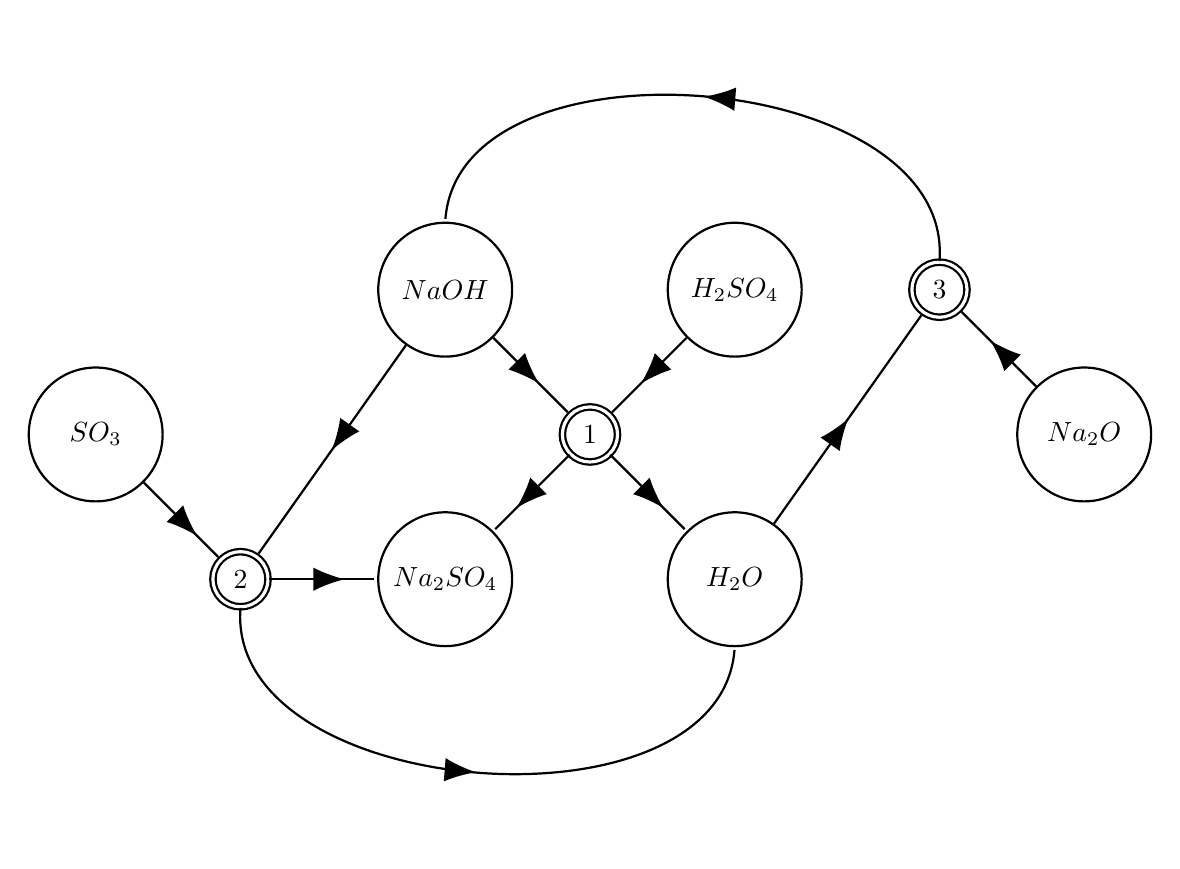
\begin{tikzpicture}[
    shorten >=1pt,
    auto,
    node distance=2.6cm,
    thick,
    compound node/.style={circle,fill=white,minimum width=1.7cm,draw},
    reaction node/.style={circle,thick,double distance=0.4mm,fill=white,minimum width=0.7cm,draw}]

  \node[compound node] (NaOH) {$NaOH$};
  \node[reaction node] (Reaction1) [below right of=NaOH] {$1$};
  \node[compound node] (H2SO4) [above right of=Reaction1] {$H_{2}SO_{4}$};
  \node[compound node] (Na2SO4) [below left of=Reaction1] {$Na_{2}SO_{4}$};
  \node[compound node] (H2O) [below right of=Reaction1] {$H_{2}O$};  
  \node[reaction node] (Reaction2) [left of=Na2SO4] {$2$};  
  \node[compound node] (SO3) [above left of=Reaction2] {$SO_{3}$};  
  \node[reaction node] (Reaction3) [right of=H2SO4] {$3$};  
  \node[compound node] (Na2O) [below right of=Reaction3] {$Na_{2}O$};  

  \path[every node/.style={font=\sffamily\small}]
    (NaOH) 
         edge[->- = .6] (Reaction1)
         edge[->- = .5] (Reaction2)
    (H2SO4) 
         edge[->- = .6] (Reaction1)
    (Reaction1) 
         edge[->- = .7] (Na2SO4)
         edge[->- = .7] (H2O)
    (SO3) 
         edge[->- = .7] (Reaction2)
    (Reaction2) 
         edge[->- = .7] (Na2SO4)
         edge[->- = .5,bend right = 90] (H2O)
    (H2O) 
         edge[->- = .5] (Reaction3)
    (Na2O) 
         edge[->- = .6] (Reaction3)
    (Reaction3) 
         edge[->- = .5,bend right = 90] (NaOH);
\end{tikzpicture}

\end{tcolorbox}

\newpage

\section{Notation}

\noindent Lets define notation, which will be helpful for description of further concepts:
\begin{itemize}

    \item Lets treat each compound type as entity from finite set: $CompoundTypes$

    \item Lets treat each reaction type as a named tuple with two attributes -- \emph{reagents} and \emph{products}. \\
             At the same time -- reagents and products will be also represented as a tuples. \\
             In general, reaction type \lq \lq$r_1 + r_2 + \cdots + r_n \rightarrow p_1 + p_2 + \cdots + p_m$\rq \rq \ -- will be represented as tuple:
             \begin{equation} \label{eq:reaction_type_notation}
                 T = (reagents:(r_1, r_2, \cdots , r_n),\ products:(p_1, p_2, \cdots , p_m))
             \end{equation}
             Where: $r_i \in CompoundTypes$ ($\forall i \in [1, n]$), and $p_j \in CompoundTypes$ ($\forall j \in [1, m]$) \\ \\
             So, lets treat all reaction types as finite set of described tuples: $ReactionTypes$

    \item Imagine, that we have reaction type $T$ (such, that $T \in ReactionTypes$). \\
             Lets use following notation for accessing to compound type of $k$-th reagent of $T$:
             \begin{equation} \label{eq:access_reagent_type_notation}
                 r_k = reagent_k(T)
             \end{equation}   
             And the similar notation for accessing to compound type of $n$-th product of $T$:
             \begin{equation} \label{eq:access_product_type_notation}
                 p_n = product_n(T)
             \end{equation}   
             Where: $p_n, r_k \in CompoundTypes$

\end{itemize}

\begin{tcolorbox}[colback=gray!5,colframe=gray!70,title=Examples of usage of described notation,left=7pt, right=7pt]
    \begin{itemize}
        \item Set of compound types might be defined as: $CompoundTypes = \{Base, Water, Acid, Salt\}$
        \item According to described notation, reaction type \lq \lq$Base + Acid \rightarrow Salt + Water$\rq \rq \ represented as: \\
                $T = (reagents: (Base, Acid),\ products: (Salt, Water))$
        \item Compound type of first reagent: $r_1 = reagent_1(T) = Base$
        \item Compound type of second product: $p_2 = product_2(T) = Water$
    \end{itemize}
\end{tcolorbox}

\section{Properties of chemical reactions graph}

As far as each chemical compound must be of some of compound types: this means, that each \emph{compound node from graph -- implicitly belongs to some compound type}. The same statement (about implicit correspondence to reaction type) is also true for \emph{reaction nodes}. 

In other words, \emph{each node of graph associated with discrete-valued random variable}: $X_i$, which corresponds either to compound type or reaction type: $x_i$ (where: $x_i \in CompoundTypes \cup ReactionTypes$). This can be represented using notation: $X_i = x_i$. 

\begin{tcolorbox}[colback=gray!5,colframe=gray!70,title=Examples of usage of described notation,left=7pt, right=7pt]
For example, imagine node of graph, which corresponds to chemical compound $NaOH$, so, the possible affiliation of given compound node to type \lq \lq $Base$\rq \rq, might be denoted as: $X_{NaOH} = Base$.
\end{tcolorbox}

In general, we will use following notation for describing probability of some specific configuration of node types of entire graph: 
\begin{equation} \label{eq:probability_notation}
P(X_1 = x_1, X_2 = x_2, \cdots , X_n = x_n) = P(x_1, x_2, \cdots , x_n) = P(x)
\end{equation}

Without loss of generalization -- we can state, that \emph{type of chemical compound depends only on types of reactions, in which given compound participates} (and vice versa -- type of chemical reaction depends only on types of compounds, which participate in given reaction).  

Such property of graph of chemical reactions might be formalized as -- \emph{conditional independence of random variables of non-adjacent nodes}.

\begin{tcolorbox}[colback=gray!5,colframe=gray!70,title=Example,left=7pt, right=7pt]

Having information -- that compound $X$ participates in reactions of following types:
\begin{enumerate}
    \item \lq \lq $Acidic\ Oxide + Basic\ Oxide \rightarrow Salt$\rq \rq
    \item \lq \lq $Basic\ Oxide + Water \rightarrow Base$\rq \rq
\end{enumerate}
We can easily \emph{infer} type of compound $X$: 
\begin{itemize}
    \item For the first type of reaction -- set of possible compound types is: \\
             $T_1 = \{Acidic\ Oxide, Basic\ Oxide, Salt\}$
    \item For the second type of reaction -- set of possible compound types is: \\
             $T_2 = \{Basic\ Oxide, Water, Base\}$
\end{itemize}
So, the type of compound $X$ is $T_1 \cap T_2 = \{Basic\ Oxide\}$

\end{tcolorbox}

Additionally -- lets temporarily assume, that all edges of reactions graph are undirected (a bit later, we will introduce this property again). \\

Considered properties of graph, leads to understanding that actually reactions graph can be treated as a \emph{\textbf{Markov Random Field}} \cite{wikipedia_mrf}.
\\

Using result of Hammersley-Clifford Theorem, we can follow up, that probability distribution of configurations of graph -- can be factorized into positive functions defined on cliques that cover all the nodes and edges (also called a \emph{Gibbs distribution})\cite{hammersley_clifford_proof, wikipedia_hammersley_clifford}:

\begin{equation}
P(x) = {1 \over Z} \prod_{c \in C_G} \psi_{c}(x_c)
\end{equation}
where:
\begin{itemize} 
    \setlength \itemsep{0em}
    \item $Z$ -- normalization constant
    \item $x$ -- configuration of node types of entire graph, as described in equation \eqref{eq:probability_notation}
    \item $C_G$ -- set of all cliques of graph
    \item $x_c$ -- configuration of node types, which belongs to clique $c$ ($x_c$ is subset of $x$)
    \item $\psi_{c}$ -- non-negative, finite functions, defined on random variables of each clique $c$
\end{itemize}

\noindent As far as graph of chemical reactions is bipartite graph -- this mean, that maximum clique size is 2. Taking into account absence of edges between nodes of the same kind -- it is clear that \emph{all cliques contain one reaction node, and one compound node (either reagent, or product)}. So, actually, for each clique we have function of 2 random variables: $\psi_c(x_i, x_j)$, where $x_i \in CompoundTypes$ and $x_j \in ReactionTypes$. So, we can rewrite \emph{joint probability} as:

\begin{equation} \label{eq:pairwise_gibbs_distribution}
P(x) = {1 \over Z} \prod_{(i,j) \in A_G} \psi_{c}(x_i, x_j)
\end{equation}
Where: $A_G$ -- is set of tuples $(i,j)$, which represents indices of adjacent nodes of chemical reactions graph. \\

As you remember -- we temporarily assumed that all edges of graph are undirected. So, lets return back this property to our graph. It can be done in very easy way -- by introducing \textbf{different kinds of clique functions}: \emph{reagent-reaction} and \emph{reaction-product} functions: $\psi_{reagent}(x_i, x_j)$ and $\psi_{product}(x_m, x_k)$ (where $x_i, x_m \in CompoundTypes$, and $x_j, x_k \in ReactionTypes$)\footnote{The similar trick was described in \cite{fraud_detection}.}. So, actually, we can express joint probability of reactions graph as:

\begin{equation}
P(x) = {1 \over Z} \left( \prod_{(i,j) \in A_R} \psi_{r}(x_i, x_j) \right) \left( \prod_{(m,k) \in A_P} \psi_{p}(x_m, x_k) \right)
\end{equation}
Where:
\begin{itemize}
    \setlength \itemsep{0em}
    \item $\psi_{r}$ -- shortened notation for $\psi_{reagent}$
    \item $\psi_{p}$ -- shortened notation for $\psi_{product}$
    \item $A_R$ -- set of tuples $(i,j)$, which represents indices of nodes of \emph{reagent-reaction} cliques
    \item $A_P$ -- set of tuples $(m,k)$, which represents indices of nodes of \emph{reaction-product} cliques
    \item $A_R \cup A_P = A_G$ (where, $A_G$ -- from description of equation \eqref{eq:pairwise_gibbs_distribution})
\end{itemize}

Additionally, lets extend graph of chemical reactions by adding new kind of nodes, which explicitly represents \emph{real states} of existing nodes: $y_i$. Lets call such nodes: \emph{observed state nodes}. After this extension -- each \emph{compound node} and each \emph{reaction node} will be connected with its own \emph{observed state node}, and reactions graph -- become tripartite graph (thought the mixamum clique size: 2 -- will not change).

For this new kind of clique -- lets introduce separate kind of clique function: $\psi_{observed}(x_i, y_i)$. As far, as each observed node is uniquely connected to only one compound (or reaction) node -- lets introduce shortened notation: $\psi_{observed}(x_i, y_i) = \phi(x_i)$ -- this function can be treated as probability of belonging of compound (reaction) $X_i$ to compound- (reaction-) type $x_i$.

So, joint probability of configurations of graph can be expressed as:

\begin{equation}
    \begin{split}
    P(x) &= {1 \over Z} \left( \prod_{i \in G} \psi_{observed}(x_i, y_i) \right) \left( \prod_{(i,j) \in A_R} \psi_{r}(x_i, x_j) \right) \left( \prod_{(m,k) \in A_P} \psi_{p}(x_m, x_k) \right) \\
            &= {1 \over Z} \left( \prod_{i \in G} \phi(x_i) \right) \left( \prod_{(i,j) \in A_R \cup A_P} \psi(x_i, x_j) \right)
    \end{split}
\end{equation}
% Centering of equation with cases: http://tex.stackexchange.com/questions/27560/is-there-a-cases-environment-in-text-mode
Where:  
\begin{itemize}
    \item 
    $ 
    \psi(x_i, x_j)= 
    \begin{dcases}
        \psi_p(x_i, x_j),& \text{if } (i, j) \in A_P \\
        \psi_r(x_i, x_j) & \text{if } (i, j) \in A_R
    \end{dcases}
    $
    
    \item $G$ -- set of indices of compound and reaction nodes of reactions graph \\
\end{itemize}

\begin{tcolorbox}[colback=gray!5,colframe=gray!70,title=Example of factorized chemical reactions graph,left=7pt, right=7pt]
%\small

\begin{center}
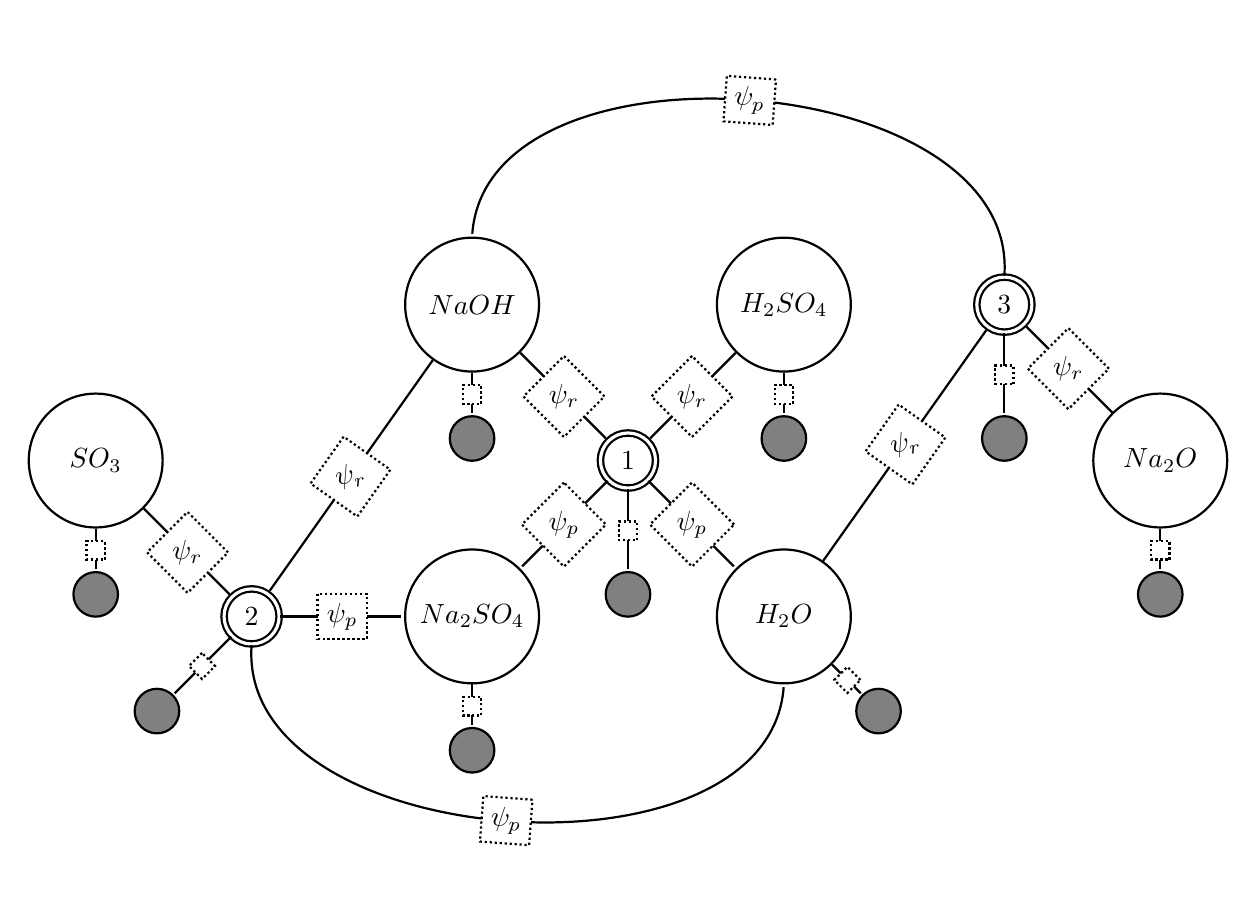
\begin{tikzpicture}[
    %scale=0.9, every node/.style={scale=0.9},
    -{Latex[length=3mm]},
    shorten >=1pt,
    auto,
    node distance=2.8cm,
    thick,
    compound node/.style={circle,fill=white,minimum width=1.7cm,draw},
    reaction node/.style={circle,thick,double distance=0.4mm,fill=white,minimum width=0.7cm,draw},
    observed node/.style={circle,draw=black,fill=gray,inner sep=.2cm, node distance = 1.7cm,outer sep=0},
    factor/.style={densely dotted, draw=black, align=center,fill=white,auto=false,sloped}]

  \node[compound node] (NaOH) {$NaOH$};
  \node[reaction node] (Reaction1) [below right of=NaOH] {$1$};
  \node[compound node] (H2SO4) [above right of=Reaction1] {$H_{2}SO_{4}$};
  \node[compound node] (Na2SO4) [below left of=Reaction1] {$Na_{2}SO_{4}$};
  \node[compound node] (H2O) [below right of=Reaction1] {$H_{2}O$};  
  \node[reaction node] (Reaction2) [left of=Na2SO4] {$2$};  
  \node[compound node] (SO3) [above left of=Reaction2] {$SO_{3}$};  
  \node[reaction node] (Reaction3) [right of=H2SO4] {$3$};  
  \node[compound node] (Na2O) [below right of=Reaction3] {$Na_{2}O$};
  
  \node[observed node] (ObservedNaOH) [below of=NaOH] {};
  \node[observed node] (ObservedH2SO4) [below of=H2SO4] {};
  \node[observed node] (ObservedNa2SO4) [below of=Na2SO4] {};
  \node[observed node] (ObservedH2O) [below right of=H2O] {};
  \node[observed node] (ObservedNa2O) [below of=Na2O] {};
  \node[observed node] (ObservedSO3) [below of=SO3] {};
  \node[observed node] (ObservedReaction1) [below of=Reaction1] {};
  \node[observed node] (ObservedReaction2) [below left of=Reaction2] {};
  \node[observed node] (ObservedReaction3) [below of=Reaction3] {};

  \path[-]
    (NaOH) 
         edge node[factor] {\rotatebox{45}{$\psi_r$}} (Reaction1)
         edge node[factor] {\rotatebox{-45}{$\psi_r$}} (Reaction2)
         edge node[factor] {} (ObservedNaOH)
    (H2SO4) 
         edge node[factor] {\rotatebox{-45}{$\psi_r$}} (Reaction1)
         edge node[factor] {} (ObservedH2SO4)
    (Reaction1) 
         edge node [factor] {\rotatebox{-45}{$\psi_p$}} (Na2SO4)
         edge node [factor] {\rotatebox{45}{$\psi_p$}} (H2O)
         edge node[factor] {} (ObservedReaction1)
    (SO3) 
         edge node [factor] {\rotatebox{45}{$\psi_r$}} (Reaction2)
         edge node[factor] {} (ObservedSO3)
    (Reaction2) 
         edge node [factor] {$\psi_p$} (Na2SO4)
         edge [bend right = 90] node [factor] {$\psi_p$} (H2O)
         edge node[factor] {} (ObservedReaction2)
    (H2O) 
         edge node [factor] {\rotatebox{-45}{$\psi_r$}} (Reaction3)
         edge node[factor] {} (ObservedH2O)
    (Na2O) 
         edge node [factor] {\rotatebox{45}{$\psi_r$}} (Reaction3)
         edge node[factor] {} (ObservedNa2O)
    (Reaction3) 
         edge [bend right = 90] node [factor] {$\psi_p$} (NaOH)
         edge node[factor] {} (ObservedReaction3)
    (Na2SO4)
         edge node[factor] {} (ObservedNa2SO4);

\end{tikzpicture}
\end{center}
$CompoundTypes = \{Base, Acid, Salt, Water, Basic\ Oxide, Acidic\ Oxide, \ldots \}$ \\ \\
$ReactionTypes = \{T_1, T_2, T_3, \ldots \}$ \\
%Where: 
%\begin{itemize}
%    \setlength \itemsep{0em}
%    \item $T_1 = (reagents:(Base, Acid),\ products:(Salt, Water))$
%    \item $T_2 = (reagents:(Basic\ Oxide, Water),\ products:(Base))$
%    \item $T_3 = (reagents:(Acidic\ Oxide, Water),\ products:(Acid))$ \\
%\end{itemize}

Lets write equation for joint probability of one of possible configurations of reactions graph:
\begin{equation*}
\begin{aligned}
        P(x) & = & P( & X_{H_2SO_4} = Acid,\ X_{Na_2SO_4} = Salt,\ X_{Na_2O} = Basic\ Oxide,\ X_{SO_3} = Acidic\ Oxide, \\
                &    &     & X_{H_2O} = Water,\ X_{NaOH} = Base,\ X_{Reaction_1} = T_1,\ X_{Reaction_2} = T_2,\ X_{Reaction_3} = T_3) = \\
                & = & {1 \over Z} & \times \phi_{NaOH}(Base) \times \phi_{H_2SO_4}(Acid) \times \phi_{Na_2SO_4}(Salt) \times \phi_{H_2O}(Water) \times \phi_{SO_3}(Acidic\ Oxide) \times \\ 
                &    &                   & \times \phi_{Na_2O}(Basic\ Oxide) \times \phi_{Reaction_1}(T_1) \times \phi_{Reaction_2}(T_2) \times \phi_{Reaction_3}(T_3) \times \\[4pt]
                &    &                   & \times \psi^{product}_{NaOH\ in\ Reaction_3}(Base,\ T_3) \times \psi^{reagent}_{Na_2O\ in\ Reaction_3}(Basic\ Oxide,\ T_3) \times \\[4pt]
                &    &                   & \times \psi^{reagent}_{NaOH\ in\ Reaction_1}(Base,\ T_1) \times \psi^{reagent}_{H_2SO_4\ in\ Reaction_1}(Acid,\ T_1) \times  \\[4pt]
                &    &                   & \times \psi^{product}_{Na_2SO_4\ in\ Reaction_1}(Salt,\ T_1) \times \psi^{reagent}_{NaOH\ in\ Reaction_2}(Base,\ T_2) \times \\[4pt]
                &    &                   & \times \psi^{product}_{Na_2SO_4\ in\ Reaction_2}(Salt,\ T_2) \times \psi^{product}_{H_2O\ in\ Reaction_2}(Water,\ T_2) \times \\[4pt]                
                &    &                   & \times \psi^{product}_{H_2O\ in\ Reaction_1}(Water,\ T_1) \times \psi^{reagent}_{H_2O\ in\ Reaction_3}(Water,\ T_3) \times \\[4pt]
                &    &                   & \times  \psi^{reagent}_{SO_3\ in\ Reaction_2}(Acidic\ Oxide,\ T_2) \\
\end{aligned}
\end{equation*}

%\normalsize
\end{tcolorbox}

\newpage

\begin{thebibliography}{9}

\bibitem{project_on_github}
  \url{https://github.com/lagodiuk/java-loopy-belief-propagation}.

\bibitem{fraud_detection}
  Leman Akoglu, Rishi Chandy, Christos Faloutsos,
  \emph{Opinion Fraud Detection in Online Reviews by Network Effects}.

\bibitem{understanding_bp}
  Jonathan S. Yedidia, William T. Freeman, and Yair Weiss,
  \emph{Understanding Belief Propagation and its Generalizations},
  TR2001-22, 
  November 2001.
  
\bibitem{wikipedia_mrf}
  \url{http://en.wikipedia.org/wiki/Markov_random_field#Definition}.
  
\bibitem{hammersley_clifford_proof}
  Samson Cheung,
  \emph{Proof of Hammersley-Clifford Theorem},
  \url{http://web.kaist.ac.kr/~kyomin/Fall09MRF/Hammersley-Clifford_Theorem.pdf},
  February 3, 2008.

\bibitem{wikipedia_hammersley_clifford}
  \url{http://en.wikipedia.org/wiki/Hammersley-Clifford_theorem}.

\end{thebibliography}

\end{document}